\section[More Modeling of Mechanical Energy Systems]{Practicing Graphical and Quantitative Modeling of Mechanical Energy Systems}
%\section{Follow-up of Module 2.2-2.3 FNTs}
\label{act2.3.2}

\begin{overview}

\textbf{Overview:} Before we introduce a new class of physical phenomena, \textbf{\emph{forces}}, we want to make sure you get a bit more practice modeling phenomena using the tools we have accumulated until now, especially the method of graphing energy amounts introduced in the last activities and the carefully crafted model-based, scientific arguments we've been practicing for a while.
	
\end{overview}

\subsection*{We've done a practice activity like this before:}

At home, please work through all the FNTs listed in this activity. In class, each group will work on a portion of these FNTs to come to a consensus before we discuss the scenarios with the whole class.\\

\begin{fnt}
	\label{fnt2.2.3-1}

This FNT is excellent practice in constructing a scientific argument based on logic that follows directly from the physical situation and the relationships of the models you use to, well, model the situation. This is what science is all about!\\

\noindent Please refer back to \hyperref[act2.2.3]{Activity~\ref*{act2.2.3}}:

\begin{enumerate}[(a)]
	\item Finish any of the prompts from \ref{act2.2.3-2} and \ref{act2.2.3-3} that you were unable to finish during the last discussion lab.
	\label{fnt2.2.3-1a}
	
	\item  Respond to the prompt in \ref{act2.2.3-4}, which asks you to turn your responses to prompts from \ref{act2.2.3-2} and \ref{act2.2.3-3} into a set of statements that constitute a logical argument based on the \EnergyInteractionModel{}.
	
		With your argument, explain why the set of masses with smaller total mass moves faster than the set with greater total mass as long as the difference between the two masses in each set is the same.
	\label{fnt2.2.3-1b}
\end{enumerate}
\end{fnt}

\begin{fnt}
	\label{fnt2.2.1-7}

A \unit[0.4]{kg} mass is attached to a spring that can compress as well as stretch (spring constant \unitfrac[50]{N}{m}). The mass and spring are resting on a horizontal tabletop. The mass is pulled, stretching the spring \unit[48]{cm}. When it is released, the system begins to oscillate.

\begin{enumerate}[(a)]
	\item\label{fnt2.2.1-7a} Assuming the transfer of energy to thermal energy systems is negligible, construct a complete \EnergyDiagram{} that could be used to predict the speed of the mass as it passes a point that is a distance of \unit[39]{cm} from its equilibrium point on the other side of the equilibrium position (spring is compressed).
	
		Substitute all known values of constants and variables into the algebraic expression of energy conservation, and identify any unknown(s). Do you have enough information to find the speed of the mass?
	
	\item\label{fnt2.2.1-7b} Now assume that the effects of friction are not negligible. When pulled back and released as before, the mass now reaches its furthest distance from equilibrium at \unit[40]{cm} on the compressed side (before bouncing back again). Construct a complete \EnergyDiagram{} that could be used to determine the amount of energy transferred to thermal systems when going from the initial stretched position to where it first momentarily stops.
	
		\textbf{Proceed as in part a:} Substitute all known values and identify any unknown(s). Can you determine the increase in thermal energy?
\end{enumerate}
\end{fnt}

\begin{fnt}
	\label{fnt2.2.1-8}

\begin{wrapfigure}{R}{.28\textwidth}
	\vspace{-15pt}
  	\centering
	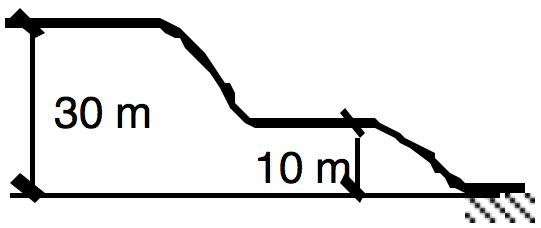
\includegraphics[width=0.95\linewidth]{fnt221-8-hill}
	\vspace{-10pt}
\end{wrapfigure}

A skier (of mass \unit[55]{kg}) skies down the smooth (frictionless) ski slope illustrated in the cross-sectional diagram. She pushes off at the top with a speed of \unitfrac[10]{m}{s}. At the bottom (\unit[0]{m}), she comes to a stop by digging her skis in sideways.

\begin{enumerate}[(a)]
	\item\label{fnt2.2.1-8a} Construct a complete \EnergyDiagram{} that can be used to predict the speed of the skier when she is on the middle flat part (at \unit[10]{m}). Substitute all known values of constants and variables, and identify any unknown(s). Do you have enough information to determine the speed at this part of the hill?

	
	\item\label{fnt2.2.1-8b} Construct a complete \EnergyDiagram{} that can be used to predict the skier's maximum speed just before digging in her skis at the bottom. Substitute for constants and variables and identify any unknown(s) as in Part~\eqref{fnt2.2.1-8a}.

	
	\item\label{fnt2.2.1-8c} Assuming that the snow at the point where she comes to a stop is at a temperature of \unit[0]{\textdegree{}C} and that all of the kinetic energy of the skier goes into melting the snow, construct a complete \EnergyDiagram{} that can be used to predict the amount of snow melted by the skier while stopping. Substitute for constants and variables and identify any unknown(s) as in Part~\eqref{fnt2.2.1-8a}.
\end{enumerate}

\end{fnt}

\begin{fnt}
	\label{fnt2.3.1-1}

\noindent Christine (from \hyperref[act2.2.1b]{Activity~\ref*{act2.2.1b}}) throws a \unit[300]{g} ball straight up into the air. The ball is exactly \unit[2]{m} above the ground when Christine lets go of it. It reaches a height \unit[12]{m} above the height from which it was released, and then falls straight back down.

\begin{enumerate}[(a)]
	\item\label{fnt2.3.1-1a} Assume that $y = 0$ at the point of release of the ball. Find the maximum and minimum values of $y$ and $PE_\text{gravity}$.
	
		What is the total energy of the system? Find the maximum and minimum values of $KE$.

	\item\label{fnt2.3.1-1b} Repeat Part~\eqref{fnt2.3.1-1a}, with $y = 0$ at the ground.	
\end{enumerate}
\end{fnt}

\begin{fnt}
	\label{fnt2.3.1-2}

A \unit[200]{g} mass is attached to a spring, just like in \hyperref[SpringMassActivity]{Activity~\ref{SpringMassActivity}}. The mass is lifted up \unit[5]{cm} and released so that it begins to oscillate about the equilibrium point. The spring has a spring constant $k = \unitfrac[500]{N}{m}$ ($= \unitfrac[500]{J}{m^2}$).

\begin{enumerate}[(a)]
	\item Calculate and accurately plot on a letter size ($\unit[8.5 \times 11]{in}$) sheet of graph paper $PE_\text{spring-mass}$, $E_\text{total}$, and $KE$. The vertical axis of the graph should be energy (in Joules). The horizontal axis is ``distance from equilibrium'' (in Meters). 

	\item On the same graph, quickly sketch (without calculating values) the $PE_\text{spring-mass}$, $KE$ and $E_\text{total}$ of the system if the mass were initially pulled back (stretched) \unit[2.5]{cm} from its equilibrium point, instead of lifted up (compressed) \unit[5]{cm}.
\end{enumerate}
\end{fnt}

\begin{fnt}
	\label{fnt2.3.1-3}

Remember the physical situation described in \ref{fnt2.2.1-8}? To refresh your memory:\\

\begin{wrapfigure}{R}{.28\textwidth}
	\vspace{-15pt}
  	\centering
	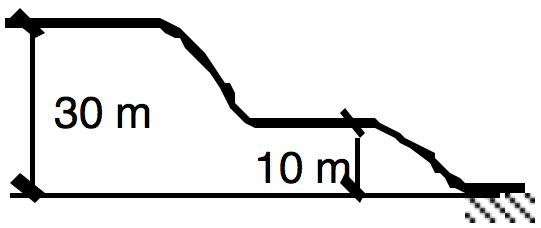
\includegraphics[width=0.95\linewidth]{fnt221-8-hill}
	\vspace{-10pt}
\end{wrapfigure}

\noindent A skier (of mass \unit[55]{kg}) skies down the smooth (frictionless) ski slope illustrated in the cross-sectional diagram. She pushes off at the top with a speed of \unitfrac[10]{m}{s}. At the bottom (\unit[0]{m}), she comes to a stop by digging her skis in sideways.\\

\noindent Use the algebraic expression of energy conservation that shows that the sum of all the energies at all points in time is constant and equal to the total energy for the following:

\begin{enumerate}[(a)]

	\item Pick a location to set $y = 0$ and determine the total energy of the system.
	\item Write an algebraic representation expressing energy conservation that you could use to find the speed of the skier when she is on the middle flat part (at the height \unit[10]{m}).
	\item Substitute all known values of constants and variables, and identify any unknown(s).
	
\end{enumerate}

\end{fnt}

\begin{center}\noindent\textbf{Each group is responsible for putting one of the following on the board.\\ Write so that all other groups can easily follow your presentation!}\end{center}

\noindent\framebox[1.1\width][c]{\textbf{Group 1}}\\

\noindent\ref{fnt2.3.1-1}\\

\noindent For each of Parts~\eqref{fnt2.3.1-1a} and \eqref{fnt2.3.1-1b} of this FNT, make a simple sketch (not a graph) showing the origin 
(where $y = 0$), the ball's initial position, positions $y_\text{max}$ and $y_\text{min}$, and the floor. Then, for each of your two sketches, show how to find the maximum and minimum values of gravitational potential energy, and the total energy.\\

\noindent Be ready to explain how changing the location of where $y = 0$ will affect $PE_\text{gravity}$.\\

\noindent\framebox[1.1\width][c]{\textbf{Group 2}}\\

\noindent\ref{fnt2.3.1-2}

\begin{enumerate}[(a)]
	\item Draw $PE_\text{spring-mass}$ and $E_\text{total}$ (but not $KE$) on a graph of Energy vs.\ ``Distance ($x$) from equilibrium'' for the case of the mass displaced \unit[5]{cm} from equilibrium and released. Clearly label the maximum and minimum values of $PE_\text{spring-mass}$.
	
	\item Demonstrate how to use point by point plotting to graph the $KE$ by doing the following: For at least two different values of $x$, use energy conservation in the form: ``$KE = E_\text{total} - PE$'' to plot a point representing the $KE$. Label the graph clearly showing $PE$, $E_\text{total}$, and $KE$ at each point. In the Whole Class Discussion you can show how to then fill in the $KE$ by sketching a dashed line connecting the points with a smooth curve.
	
	\item On the same graph, quickly draw $PE_\text{spring-mass}$ and $E_\text{total}$ (but not $KE$) for the case of the mass displaced \unit[2.5]{cm} from equilibrium.
\end{enumerate}

\noindent\framebox[1.1\width][c]{\textbf{Group 3}}\\

\noindent\hyperref[fnt2.2.1-7a]{\ref*{fnt2.2.1-7} Part~\ref*{fnt2.2.1-7a}}\\

\noindent Construct a complete \EnergyDiagram{} with accompanying equations as directed in Part~\eqref{fnt2.2.1-7a} of this FNT, and be ready to explain if you have enough information to determine the speed of the mass.\\

\noindent\hyperref[fnt2.2.1-7b]{\ref*{fnt2.2.1-7} Part~\ref*{fnt2.2.1-7b}}\\

\noindent Construct a complete \EnergyDiagram{} with accompanying equations as directed in Part~\eqref{fnt2.2.1-7b} of this FNT, and be ready to explain if you have enough information to determine the increase in thermal energy.\\
 
\noindent\framebox[1.1\width][c]{\textbf{Group 4}}\\

\noindent\hyperref[fnt2.2.1-8a]{\ref*{fnt2.2.1-8} Part~\ref*{fnt2.2.1-8a}}\\

\noindent Construct a complete \EnergyDiagram{} with accompanying equations as directed in Part~\ref*{fnt2.2.1-8a} of this FNT, and be ready to explain if you have enough information to determine the speed of the skier on the middle part of the hill.\\

\noindent\framebox[1.1\width][c]{\textbf{Group 5}}\\

\noindent\hyperref[fnt2.2.1-8b]{\ref*{fnt2.2.1-8} Part~\ref*{fnt2.2.1-8b}}\\

\noindent Construct a complete \EnergyDiagram{} with accompanying equations as directed in Part~\eqref{fnt2.2.1-8b} of this FNT, and be ready to explain if you have enough information to determine the speed of the skier at the bottom of the hill.\\

\noindent Could you have used different initial values of energy system indicators to answer the same question? Briefly show/explain on the board.\\

\noindent\framebox[1.1\width][c]{\textbf{Group 6}}\\

\noindent\ref{fnt2.3.1-3}\\

\noindent Put your response for this FNT on the board. Be sure to show how you determined the total energy of the physical system.\\

\noindent Is this the only correct value of total energy for the system? Briefly show/explain.\\

\noindent\framebox[1.1\width][c]{\textbf{All Groups}}\\

\noindent\ref{fnt2.2.3-1}\\

\noindent Put your response for this FNT on the board.\\

\WCD